% Created 2020-02-19 mié 08:51
\documentclass[a4paper]{scrartcl}
\usepackage[utf8]{inputenc}
\usepackage[T1]{fontenc}
\usepackage{fixltx2e}
\usepackage{graphicx}
\usepackage{longtable}
\usepackage{float}
\usepackage{wrapfig}
\usepackage{rotating}
\usepackage[normalem]{ulem}
\usepackage{amsmath}
\usepackage{textcomp}
\usepackage{marvosym}
\usepackage{wasysym}
\usepackage{amssymb}
\usepackage{hyperref}
\tolerance=1000
\usepackage{khpreamble}
\usepackage{pgfplots}
\usepackage{pdfpages}
\usepackage{circuitikz}
\usepgfplotslibrary{groupplots}
\usetikzlibrary{positioning}
\renewcommand*{\not}[1]{\ensuremath{\bar{#1}}}
\renewcommand*{\not}[1]{\ensuremath{\overline{#1}}}
\author{Kjartan Halvorsen}
\date{2020-02-19}
\title{Capacitors, RC-circuit, first-order response}
\hypersetup{
  pdfkeywords={},
  pdfsubject={},
  pdfcreator={Emacs 25.3.50.2 (Org mode 8.2.10)}}
\begin{document}

\maketitle


\section{Repetition}
\label{sec-1}
\subsection{Transforming signals}
\label{sec-1-1}
We looked last week at circuits like the one below
\begin{center}
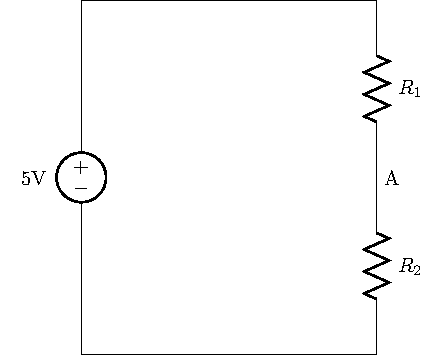
\includegraphics[width=0.4\linewidth]{../../figures/voltage-divider-circuit}
\end{center}
and we were interested in the voltage across the second resistor. A simple circuit like this may be interesting the first time you see it and measure the current and voltages, but will quickly look at bit dull. But redrawing the circuit slightly, and you may see that this is actually a very useful simple circuit for transforming signals:
\begin{center}
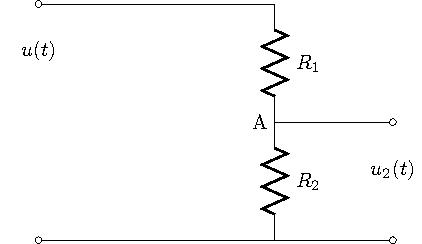
\includegraphics[width=0.4\linewidth]{../../figures/voltage-divider-input-output}
\end{center}
We can think of the input voltage $u(t)$ as an \textbf{input signal} to the circuit, and the signal $u_2(t)$ as the \textbf{output signal}. We learned from last week that
\[ u_2(t) = \frac{R_2}{R_1+R_2}u(t),\]
so the circuit can be seen as a static gain less than 1
   \begin{center}
  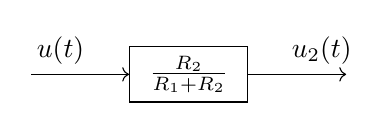
\begin{tikzpicture}[node distance=22mm, block/.style={rectangle, draw, minimum width=15mm}, sumnode/.style={circle, draw, inner sep=2pt}]
    
    \node[coordinate] (input) {};
    \node[block, right of=input, node distance=20mm] (plant)  {$\frac{R_2}{R_1+R_2}$};
    \node[coordinate, right of=plant, node distance=20mm] (output) {};

    \draw[->] (input) -- node[above, pos=0.3] {$u(t)$} (plant);
    \draw[->] (plant) -- node[above, near end] {$u_2(t)$} (output);
  \end{tikzpicture}
\end{center}

No you see that the simple voltage-divider circuit is in fact 
\section{Capacitors}
\label{sec-2}

\subsection{Current and water flow analogy}
\label{sec-2-1}
When trying to understand what is going on in electrical circuits it can be very helpful to use theintuition we have about the flow of water. All of us have a much stronger intuition for things like water pressure and flows, than we have about voltage and current. This comes from the simple fact that we observe, perceive and interact with water every single day since we were born. But we hardly ever sense or perceive voltage and electrical current (when we do it can be rather painful and something we remember for along time, though). 

   All the concepts of electricity and circuit elements we will see in this course have direct analogies in realm of fluids. Last week we worked with voltages, resistance and current. Voltage is the difference in electric potential between two points, and corresponds to the different in pressure between two bodies of water (high and low reservoirs, for instance). In fact, voltage is sometimes called \textbf{electric pressure}. Voltage is measured in Volt. 
   Electric current is a flow of charged particles. Most often these particles are electrons that can move in a conducting metal. But it can also be charged ions in an electrolytic fluid. Current is measured in Amperes. Electrical charge is a fundamental property of materia, and is measured in the unit Coulomb (C). The size of one Coulomb is related to current A. One C is the amount of charge that flows through a conductor if the current is 1A. 
A resistor is a resistance to electric current. It corresponds to a tube in a hydraulic ssystem.   There will be a pressure drop across a tube when water is flowing through it, and in the same way there is a drop in voltage across a resistor. Resistance is measured in Ohms. This units are related so that a circuit with a 1V voltage source and a 1 Ohm resistance will have a current of 1 A.

\begin{center}
\begin{tabular}{ll}
Electricity & Fluids\\
\hline
Current is flow of charged particles (electrons) & Current is flow of molecules\\
Voltage a potential difference that can move electrons & Fluids at  heights (pressure)\\
Current flows from high potential to low & Flow from higher to lower height\\
(although the electrons flow from low to high pot) & \\
A resistor connecting two potentials gives restricted flow & Tube connecting two reservoirs\\
Current must flow in loops & Not so? (to ambient)\\
Electric potential means potential to do work (run motor) & Same\\
Capacitor & Membrane in tube\\
Charge stored in capacitor & Volume of displaced membrane\\
Voltage across capacitor & Force (pressure) of membrane\\
 & In equilbrium the difference in\\
 & pressure at both sides\\
Capacitans charge/voltage & Compliance of membrane\\
\end{tabular}
\end{center}

\subsection{Working principle of capacitors}
\label{sec-2-2}
\begin{itemize}
\item Two plates (metal sheets) with non-conducting medium between.
\item Charge is accumulated on either side
\item Characterized by the potential difference (voltage across) for a given amount of charge Q.
\begin{itemize}
\item C = charge/voltage <=> C*voltage = charge <=> voltage = charge/C
\item Note that current is flow of charge, so dQ/dt = i, or Q = Q(0) + $\int$$_{\text{0}}^{\text{t}}$ i(s) ds
\item C*voltage = Q(0) + $\int$$_{\text{0}}^{\text{t}}$ i(s)ds
\end{itemize}
\end{itemize}

A capacitor is a device that stores electrical potential energy. Recall from what you know about energy: Energy existst primarily in two forms: Potential and kinetic. Potential energy has to do with position, and kinetic with movement. Think of a hydro power plant. Potential energy exists in the form of a body of water in a reservoir at an height above the turbine. The water is led in large tubes down to the turbine. When the water hits the turbine blades, they hit it at high velocity. This means that the potential energy of water at a height has been transformed into kinetic energy in the form of moving water molecules.
Continuing with the hydro-power plant analogy: Can you think of some way that kinetic energy is stored in the system?
The water molecules hit the turbine blades at high speed, and then they flow slowly out of the power plant. They make the turbine spin, so their kinetic energy is transferred to energy in the spinning turbine, where it can be expresss as E$_{\text{k}}$ = 1/2 J\dot{\theta}$^{\text{2}}$, where J is the moment of inertia of the turbine, and \dot{\theta} is the angular velocity. In steady-state the turbine rotates with a velocity corresponding to the velocity of the water. And importantly, it will oppose a change in the velocity of the water, since it cannot change velocity instantly. In fact, it follows Newton's second law J d/dt (\dot{\theta}) = $\sum$ torques. 
In electricity their exists a circuit element which has similar characteristics. It is called an \textbf{inductor}, and consists basically of a coil of wire. More on this next week.

Back to capacitors. We are all very familiar with devices that store electrical, potential, energy. We call them batteries. A capacitor is in fact like a battery, but it is typically charged and discharged much faster. A capactior is characterized by the amount of charge that is accumulated in it for each voltage difference over it (between its two legs or terminals). This value is called the \textbf{capacitans}
\[ C = \frac{\text{charge}}{\text{voltage}}. \]



Electrical energy conists in the form of
\subsection{Electrolytic capacitors}
\label{sec-2-3}
\begin{itemize}
\item Polarity. Careful!
\item Because of how they are produced cannot take potential in wrong direction (break down).
\item Think of a membrane that is strong in one direction but breaks easily in the other
\item Symbol
\end{itemize}

\section{Impedance}
\label{sec-3}

\subsection{Ohm's law (\(u=Ri\)) is static}
\label{sec-3-1}

\subsection{Capacitor equation}
\label{sec-3-2}
\[ Cu(t) = Q(0) + \int_0^t i(s) ds, \qquad \text{differentiate}\]
\[ C \dot{u}(t) = i(t) \quad \Leftrightarrow \quad \dot{u}(t) = \frac{1}{C} i(t). \]
Dynamic relationship between current and voltage! Apply Laplace trf
\[ sU(s) - u(0) = \frac{1}{C} I(s) \quad \Leftrightarrow \quad U(s) = \frac{u(0)}{s} + \frac{1}{sC} I(s). \]




\section{The RC circuit}
\label{sec-4}

\section{Simulate}
\label{sec-5}

\subsection{From "scratch"}
\label{sec-5-1}
   Start with integration:  d/dt u$_{\text{c}}$ = \frac{1}{C} i
                  volt
volt in -----> o -----
\section{Experiment}
\label{sec-6}
\subsection{Get the material}
\label{sec-6-1}

\subsection{Present the lab instructions}
\label{sec-6-2}

\subsection{Circuit and physical implementation}
\label{sec-6-3}

\begin{center}
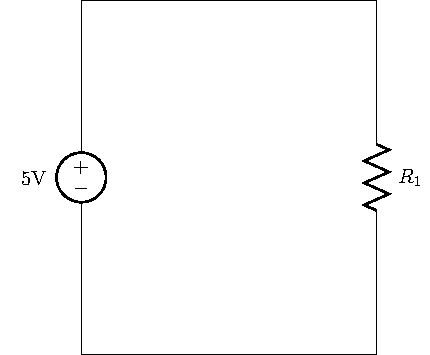
\includegraphics[width=0.4\linewidth]{../../figures/R-circuit}
Draw breadboard with resistor. Connect!
\end{center}

Describe the ideal voltage source: Will provide any current that the circuit may demand, at a perfectly constant voltage $u$. 

\subsection{Important relationsships}
\label{sec-6-4}

\subsubsection{Ohm's law}
\label{sec-6-4-1}
\(u = Ri\)

\subsubsection{Kirchoff's current law}
\label{sec-6-4-2}

\subsubsection{Kirchoff's voltage law}
\label{sec-6-4-3}

\subsection{Series connection}
\label{sec-6-5}
\begin{center}
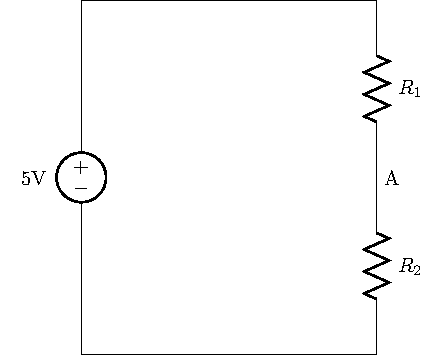
\includegraphics[width=0.4\linewidth]{../../figures/voltage-divider-circuit}
\end{center}
In the equivalent circuit with a single resistor $R_3$, then clearly $u_3=u$. And for the original circuit $u = u_1 + u_2$. The same current $i$ flows through all the elements, so from Ohm's law $u_k = R_k i_k$, we get
\( u_3 = u_1 + u_2\) and
\[ R_3 i = R_1 i + R_2 i = (R_1 + R_2) i \]
\[ R_3 = R_1 + R_2\]

This means that $i = \frac{u}{R_1 + R_2}$. So what is the voltage over $R_2$?
\[ u_2 = R_2 i = u \frac{R_2}{R_1 + R_2}. \]

\subsection{Parallel connection}
\label{sec-6-6}

\begin{center}
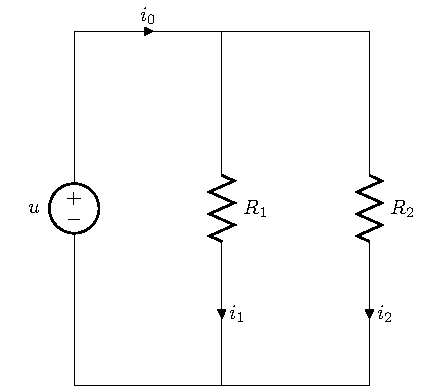
\includegraphics[width=0.4\linewidth]{../../figures/parallel-circuit}
\end{center}

In an equivalent circuit with only one resistor $R_3$, we must have \(u_3 = u = R_3 i_0\), which implies \(i_0 = \frac{u}{R_3}\).
For the two resistors in the circuit, we have \(u_1 = u = R_1 i_1\) and \(u_2 = u = R_1 i_1\), which gives \[i_1 = \frac{u}{R_1} \qquad \text{and} \qquad \(i_2 = \frac{u}{R_2}\]
From Kirchoff's current law \(i_0 = i_1 + i_2\), so  we get
\[ \frac{u}{R_3} = \frac{u}{R_1} + \frac{u}{R_2} = u \left( \frac{1}{R_1} + \frac{1}{R_2}\right)\]
hence
\[ \frac{1}{R_3} =  \frac{1}{R_1} + \frac{1}{R_2}\]
The reciprocal \(\frac{1}{R}\) of a resistance is called \emph{admittance}. 

\subsection{Safety instructions}
\label{sec-6-7}

\subsubsection{Connect everything first, then turn on the power supply}
\label{sec-6-7-1}

\subsubsection{Use low voltage, 5V}
\label{sec-6-7-2}
% Emacs 25.3.50.2 (Org mode 8.2.10)
\end{document}